\documentclass[border=0.5mm]{standalone}

\usepackage{import}
\subimport{../../../}{preamble.tex}

\usepackage{tikz}
\usetikzlibrary{calc}

\usepackage{pgfplots}
\usepgfplotslibrary{fillbetween}

\begin{document}

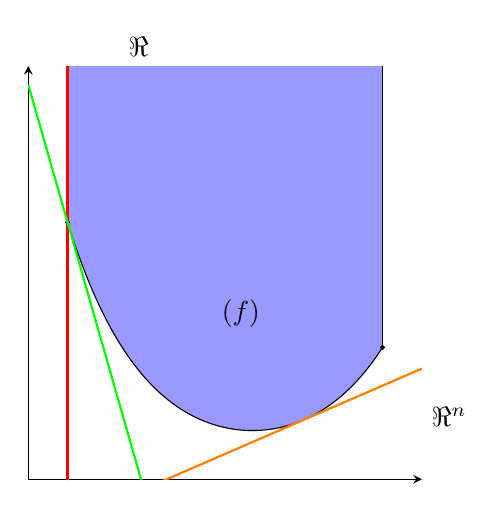
\begin{tikzpicture}

  \begin{axis}[
    ticks=none,
    axis lines=left,
    y=3.5cm,            % y unit vector
    x=1cm,            % x unit vector
    xmin=-2.5,
    xmax=2.5,
    ymin=0,
    ymax=1.5,
    clip=true,
    xlabel=$\Re^n$,
    ylabel=$\Re$,
    x label style={at={(axis description cs:1.0,0.15)},anchor=west},
    y label style={at={(axis description cs:0.23,1.0)},rotate=-90,anchor=south west},
    ]
    
    \addplot[name path=F, mark=none, black, samples=100, domain=-2:2] {(exp(-x)+exp(x)/2)/8};
    \addplot[name path=S, mark=none, draw=white, samples=10, domain=-2:2] {1.5};

    \node[fill, draw, circle, inner sep=0.5] (ub) at (axis cs:2.0, 0.47873291658774225) {};
    \draw (ub)--(axis cs:2.0, 1.5);

    \node[fill, draw, circle, inner sep=0.5] (lb) at (axis cs:-2.0, 0.9320904675686196) {};
    \draw (lb)--(axis cs:-2.0, 1.5);


    \addplot[blue!40] fill between[of=F and S];

    \node at (axis cs:0.2,0.6) {$\epi(f)$};

    \draw[red, thick] (axis cs:-2.0, 1.5)--(axis cs:-2.0, -2.5);

    \addplot[mark=none, green, thick, samples=100, domain=-2.5:2.5] {0.9320904675686196-1*(x+2)};

    \addplot[mark=none, orange, thick, samples=100, domain=-2.5:2.5] {0.2158775444251206+0.123908*(x-1)};
  \end{axis}

  
\end{tikzpicture}

\end{document}

%%% Local Variables:
%%% mode: latex
%%% TeX-master: t
%%% End:
